%%%%%%%%%%%%%%%%%%%%%%%%%%%%%%%%%%%
%%  Object identification
%%%%%%%%%%%%%%%%%%%%%%%%%%%%%%%%%%%



% The average pileup energy due to neutral hadrons is computed
% event-by-event and subtracted from the energy when computing lepton isolation and jet energy.  The
% energy subtracted is  the average pileup energy per unit area (in $\Delta\eta \times \Delta\phi$)
% times the jet area~\cite{Fastjet1, Fastjet2}.
% this corrects energy and momentum, not substructure
% TODO: move to jet and lepton sections

% 
% Missing transverse energy, which is used in the calculation of the razor variable $\mr$, is 
% defined to be the negative sum of the transverse momenta of all the particle flow objects in an
% event.  Loosely identified and isolated electrons with $\pt > 5$~\GeV and $|\eta| < 2.5$ and muons
% with $\pt > 5$\GeV and $|\eta| < 2.4$ are used both to suppress backgrounds in our signal region
%and
% in the definition of the control regions.  A tight definition of isolated leptons (electrons with
% $\pt > 10$~\GeV and $|\eta| < 2.5$ and muons with $\pt > 10$~\GeV and $|\eta| < 2.4$) defines a
% control region enriched in $\cPZ \rightarrow \ell \ell $ events, from which we estimate the
% systematic uncertainty in the predicted number of $\cPZ \rightarrow \nu \nu$ events in the signal
% region. Any electron candidates with $1.44 < |\eta| < 1.57$ are rejected since the transition
%region
% between barrel and endcap calorimeters is less well-instrumented.
% In order to suppress the decays of taus and other leptons that fail the loose selection, events
%that
% have isolated tracks with $\pt > 10$\GeV and track-primary vertex distance along the beam
%direction
% $dz < 0.05$ are rejected.

\subsubsection{Primary vertices \label{sec:object_vertex}}

We require at least one {\it good} primary vertex to be reconstructed in each event. 
This vertex should be associated with at least four charged-particle tracks. It should also lie
within 24\cm of the origin of the CMS coordinate system along the beam direction, and within 2\cm
in the plane transverse to the beam. 
These requirements, translated to the CMS nomenclature, are summarized in
Table~\ref{tab:object_vertex}.
In case there are multiple good vertices, we choose the vertex with the highest value of $\sum
\pt^2$ of associated tracks to be the leading primary vertex in the event. This vertex is
taken as a reference to reconstruct the event, e.g. to perform the track subtraction for pileup
removal, for which we use the charged hadron subtraction algorithm, as explained before.

\begin{table}[htdp]
\caption{Vertex selection criteria. \label{tab:object_vertex}}
\begin{center}
\begin{tabular}{l l}
\toprule
\texttt{\small isFake()} & $= 0$ \\
\texttt{\small ndof()} & $> 4$ \\
\texttt{\small z()} & $< 24\cm$ \\
\texttt{\small position.Rho()} & $< 2\cm$ \\
\bottomrule
\end{tabular}
\end{center}
\end{table}


\subsubsection{Jets \label{sec:object_jets}}

Most analyses are interested primarily in the quarks and gluon produced in the hard interaction, or
in the decay of heavy particles, such as top quarks or $\W$ bosons. 
However, through the process of parton showering and hadronization, the few initial quarks and
gluons turn into a multitude of hadrons. 
Hadrons from a given initial quark or gluon can usually be found close together, they form a
\textit{jet}. The proper description of jets, and the jet definitions that are used to reconstruct
them, relies on two properties: infrared, and collinear safety~\cite{Salam:2009jx}.
It is important that a jet definition returns the same set of final jets regardless of whether a
parton underwent a collinear or soft splitting. If this is not the case, i.e. the jet definition is
infrared or collinear unsafe, then one finds that divergencies in the theoretical computation of
jet cross sections do not vanish. 

A jet definition comprises two parts: the jet algorithm that defines in which order particles are
grouped together, and the recombination scheme that defines how to combine the momenta of the
to-be-merged particles. 
For the latter, the most common choice is to simply add the four-vectors of the particles, which
then gives rise to massive jets. 
For the jet algorithm there are many choices. Here I will focus solely on the anti-$k_\textrm{T}$
algorithm~\cite{antikt}, which is the default jet algorithm used by CMS.
As for most sequential recombination algorithms, one defines distances $d_{ij}$ between particles
$i$ and $j$ (or pseudojets if particles have been combined before),  and distances $d_{iB}$ between
particle $i$ and the beam.
The distance measures are in this case given by
\begin{align}
  d_{ij} &= \min \left(\frac{1}{p_{\mathrm{T,i}}^2}, \frac{1}{p_{\mathrm{T,j}}^2}\right)
\frac{\Delta R_{ij}^2}{R^2}, \\
  d_{iB} &= \frac{1}{p_{\mathrm{T,i}}^2},
\end{align}
where $\Delta R_{ij}^2 = (y_i - y_j)^2 + (\phi_i - \phi_j)^2$ and $R$ is a tuneable parameter
determining the size of the jets. The rapidity $y$ of a particle is given by,
\begin{equation}
  y = \frac{1}{2} \ln{\frac{ E + p_z }{ E - p_z }} .
\end{equation}
The jet clustering proceeds by identifying the smallest of all distances. If it is a $d_{ij}$, we
recombine particles $i$ and $j$, while if it is $d_{iB}$, we move $i$ from the list of particles to
the list of final jets. All distances are then recalculated and the procedure is repeated until no
particles are left.
The anti-$k_\textrm{T}$ algorithm results in mostly circular jets, reminiscent of the older cone jet
algorithms that are no longer used because they are not infrared and collinear safe.

The input to the jet clustering are the PF candidates that pass the charged hadron subtraction. 
The clustering itself is done with the anti-$k_\textrm{T}$ algorithm with size parameter $R=0.5$
(AK5), as implemented in \textsc{FastJet 3.0.1}~\cite{Cacciari:2011ma}.
We apply the standard loose identification criteria to the resulting jets, as defined by the
requirements listed in Table~\ref{tab:object_jets}. 

Unfortunately, the calorimeter response to incident particles is not uniform. It it, therefore, not
straightforward to translate the measured jet energy to the true particle energy, which is what we
want to use to do our analysis. A set of jet energy scale corrections -- scalings of the
jet four-momentum depending on jet \pt, $\eta$ and flavour -- are applied to both data and
simulation in order to achieve a proper mapping to the particle level. The difference between the
reconstructed and particle-level jet energy is called the \textit{offset} in what follows.
Jet energy corrections within CMS are taken care of in a sequential way, each level of correction
taking care of a different effect~\cite{JEC}. 

First, the residual effect from pileup is removed using the so-called L1 corrections. The effects
of charged hadrons from in-time pileup have already been largely reduced by the charged hadron
subtraction method. The effect of neutral particles and out-of-time pileup is removed at this stage
using a slightly modified version of the \textit{jet area method}~\cite{Fastjet1,Fastjet2}.
This method uses the effective area of the jets, $A$, multiplied by the average energy density
in the event, $\rho$, to calculate the energy to be subtracted from the jets.
Both real and simulated jets are first corrected with a $\pt$, $\eta$, and number of primary
vertices dependent offset correction determined in simulation. For data events, an additional
data/simulation scale factor is derived from ZeroBias data to correct for remaining $\eta$ dependent
discrepancies.
Figure~\ref{fig:JEC_L1} shows the size of the energy offset between reconstructed and particle level
jets, before and after the L1 corrections have been applied. A clear reduction of the overall offset
is observed. 

\begin{figure}[tpb]
  \centering
  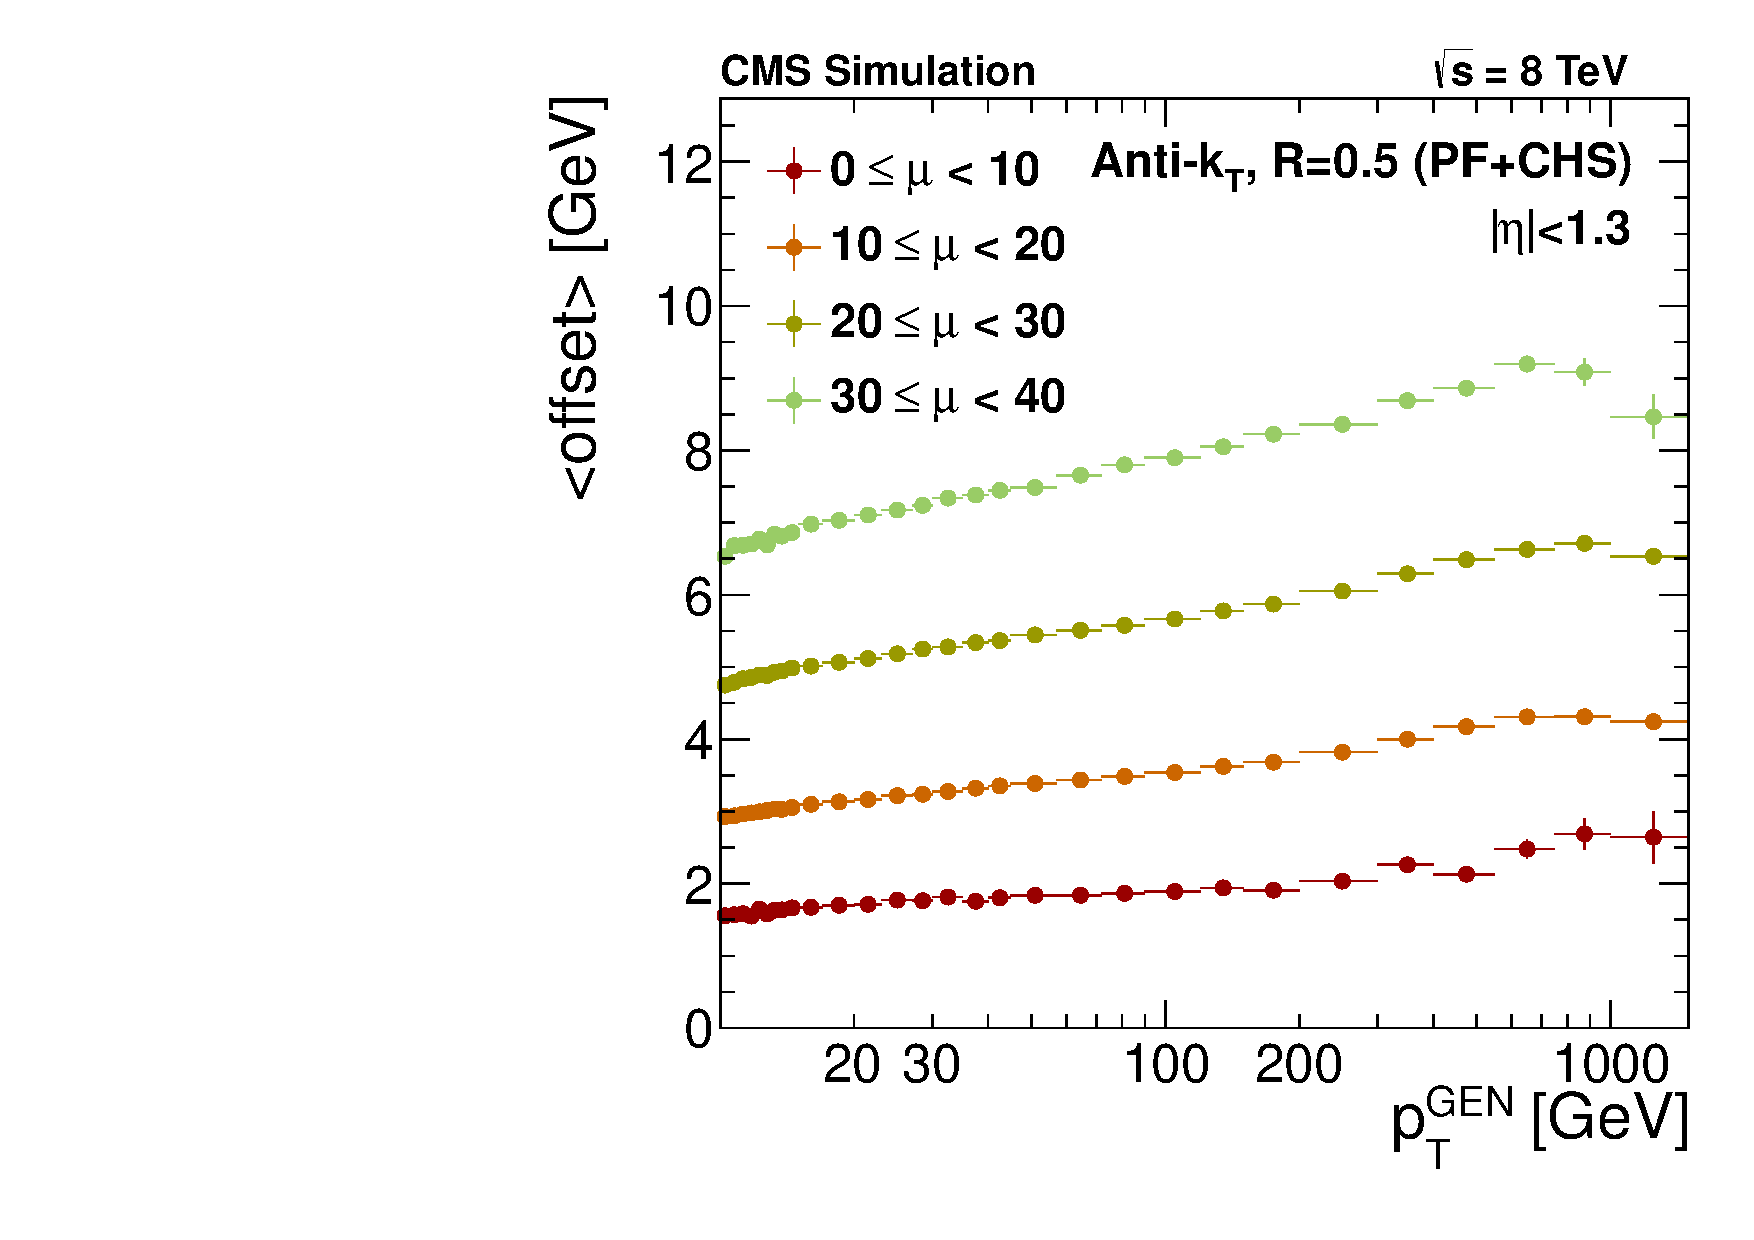
\includegraphics[width=0.4\textwidth]{figures/eventreco_objects/OffMeantnpuRef_BB_ak5pfchs}
  ~
  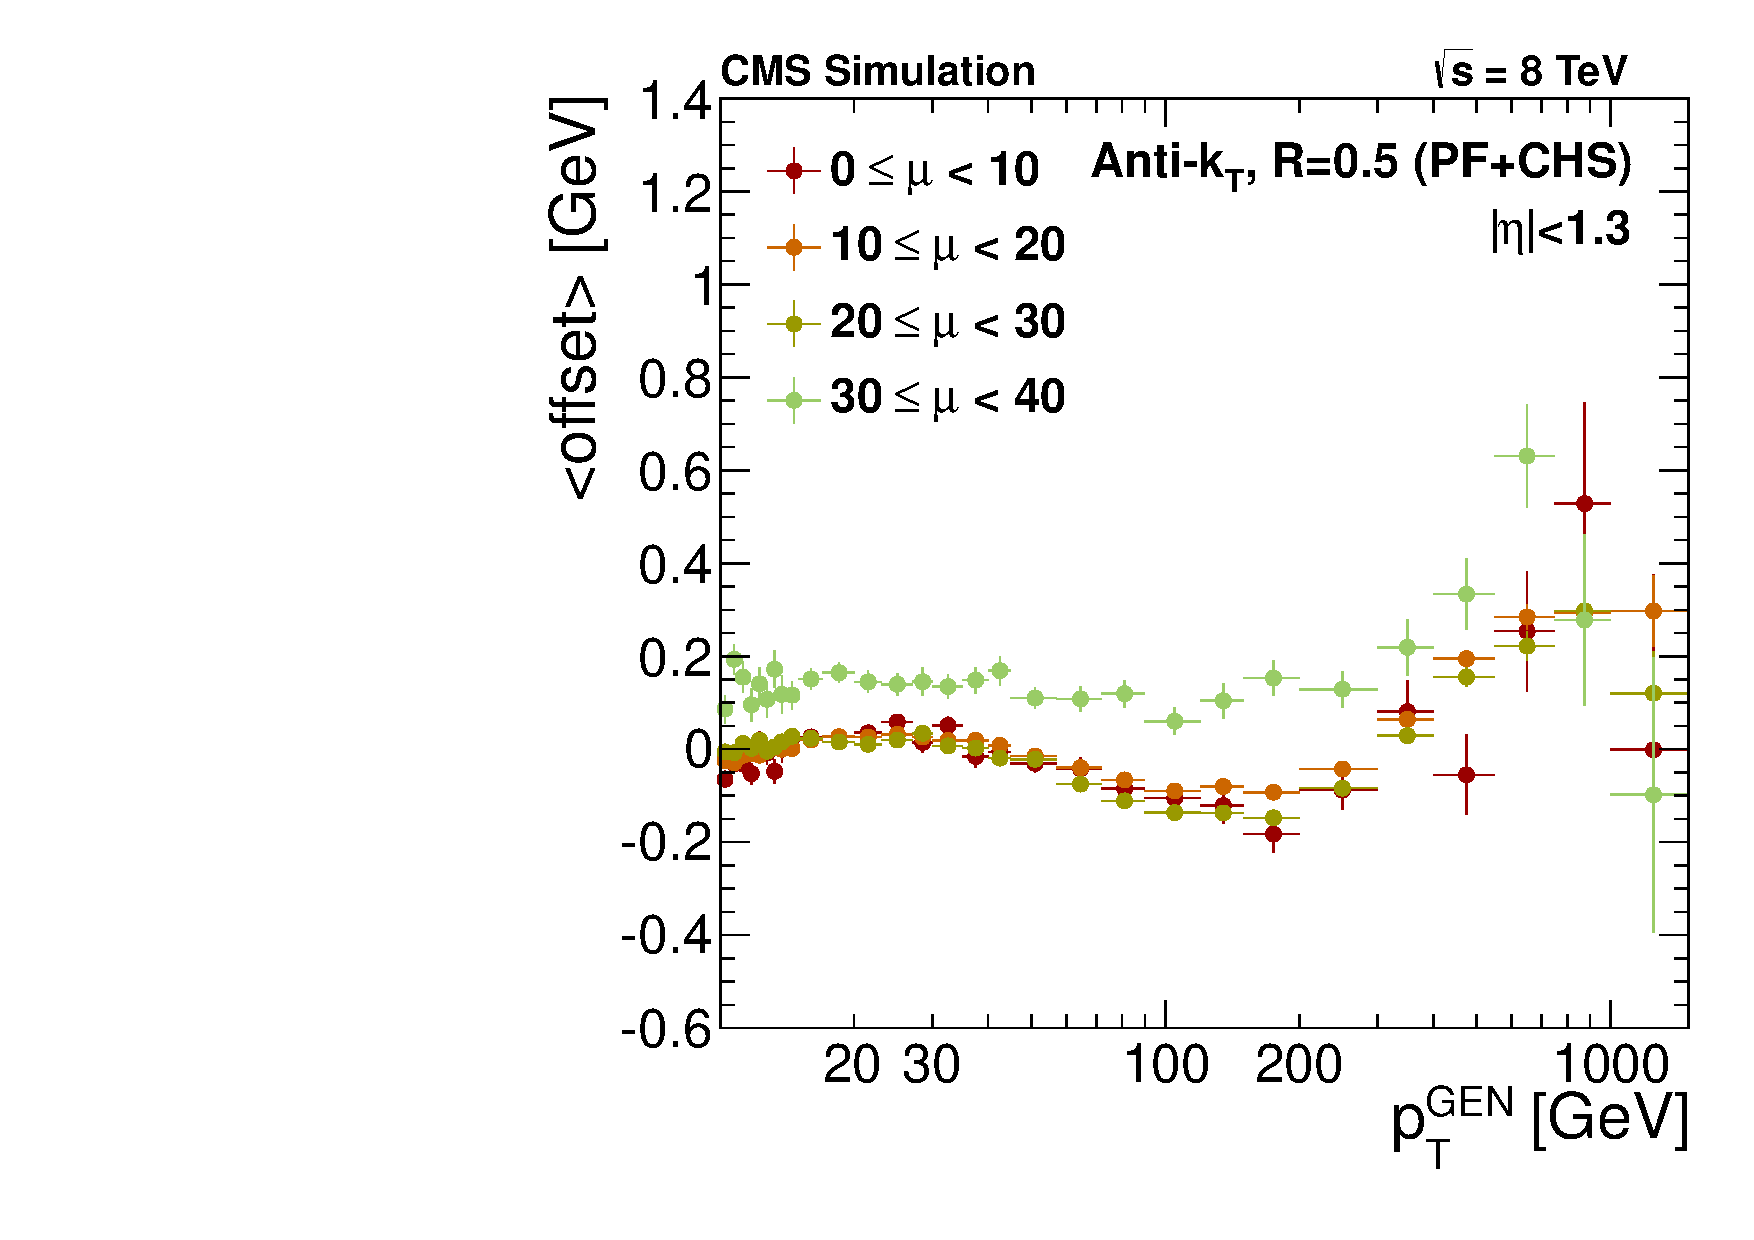
\includegraphics[width=0.4\textwidth]{figures/eventreco_objects/OffMeantnpuRef_BB_ak5pfchsl1}
  \caption{The offset shown on the $y$-axis in these plots is defined as the difference in
transverse momentum for a reconstructed jet with added pileup and the same jet without pileup.
The lefthand side shows the offset as a function of the generated \pt of a jet before the L1
corrections have been applied, and the righthand side shows the offset after pileup
corrections. Different markers represent different levels of pileup. Figures taken from
Ref.~\cite{JEC_plots}.
  \label{fig:JEC_L1}}
\end{figure}


The second level of corrections, the L2 Relative corrections, are designed to make the jet response
flat in $\eta$. Since the simulation of the detector response is very detailed, see
Section~\ref{sec:event_simulation}, the jet response is in fact very well modelled in simulation,
which is why it is used for the bulk of the jet energy corrections. 
MC truth information is used to correct a jet at arbitrary $\eta$ relative to a jet
in the central area ($|\eta|<1.3$). 

\begin{figure}[tpb]
  \centering
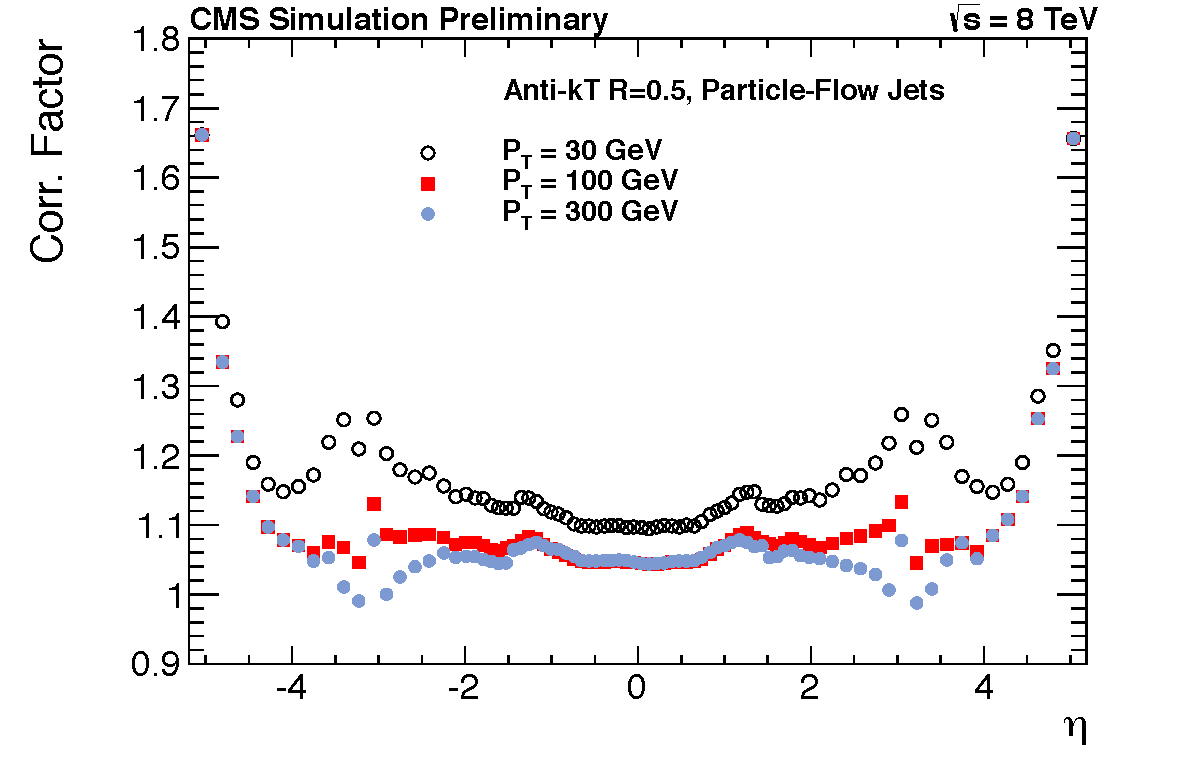
\includegraphics[width=0.6\textwidth]
{figures/eventreco_objects/CorrectionVsEta_Overview_TDR_ak5pfl1_L2L3}
  \caption{ The size of the L2 and L3 corrections as a function of jet $\eta$ for three reference
transverse momentum values: 30\GeV (white hollow circles), 100\GeV (red squares) and 300\GeV (blue
circles). Figure taken from Ref.~\cite{JEC_plots2}.
  \label{fig:JEC_L23}}
\end{figure}


Then the L3 Absolute corrections, which flatten the jet response with respect to \pt, are applied.
They are derived from simulation, and correct the jet energy back to the particle level, such that
on average the \pt of a reconstructed jet matches that of a jet clustered using generator level
particles,
\begin{equation}
  <\pt(\mathrm{reco})_{\mathrm{corr}}> {=} <\pt(\mathrm{gen})>
\end{equation}
These are the final corrections applied to jets from simulated events. 

Data events are further corrected by the L2L3 Residual jet energy scale corrections to take care of
the small differences between data and simulation. These corrections are \pt and $\eta$ dependent,
and only correct the relative energy scale. The absolute energy scale was found to be well modelled
in the simulation. A dedicated, data-driven approach is employed, using data samples of dijet,
$\gamma+$jet, and $\cPZ+$jet events. 

% TODO Add information on jet corrections and pileup subtraction


% The jets are corrected for pile-up effects in a two step process.  
% First charged hadron particle-flow candidates that have been associated with a pile-up vertex are
% removed from the list of particles to be clustered using the {\tt PFNoPileUp} algorithm.  
% The jets are then clustered and corrected for the L2 and L3 corrections, taking into
% account the charged-hadron removal. 
% The remaining PU energy is subtracted by applying the event-by-event quantity $\pi \rho (\Delta
% R)^2$, where $\Delta R$ is the jet size and $\rho$ is the average density from PU events, as
% computed by {\tt FastJet} using only neutral hadron particle-flow candidates.  

After all corrections are applied, jets are required to have $\pt > 30\GeV$ and $|\eta| < 2.4$.  

  






\begin{table}[htdp]
\caption{Jet selection criteria. \label{tab:object_jets}}
\begin{center}
\begin{tabular}{l l}
\toprule
\pt & $> 30\GeV$ \\
$|\eta|$ & $< 2.4$ \\
\midrule
\texttt{\small neutralHadronEnergyFraction()} & $< 0.99$ \\
\texttt{\small neutralEmEnergyFraction()} & $< 0.99$ \\
\texttt{\small nConstituents()} & $> 1$ \\
\texttt{\small chargedHadronEnergyFraction()} & $> 0$ \\
\texttt{\small chargedMultiplicity()} & $> 0$ \\
\texttt{\small chargedEmEnergyFraction()} & $< 0.99$ \\
\bottomrule
\end{tabular}
\end{center}
\end{table}

The AK5 jets defined here will be used for most aspects of the razor boost analysis, except for the
reconstruction of boosted hadronic $\W$-candidates. 
Section~\ref{sec:boost_wtag} provides details on the dedicated jet treatment that is used for $\W$
tagging.

\subsubsection{B-Tagging \label{sec:object_btag}}

Jets originating from the hadronization of $\cPqb$ quarks can be distinguished from other jets,
initiated by gluons or light flavor quarks, due to the long lifetime of the $\cPqb$ quark. 
The non-prompt decay of the $B$ hadrons results in a secondary vertex, displaced with respect to
the primary vertex of the hard interaction. 

% TODO add more info on b-tagging algorithm

The ability to distinguish $\cPqb$ jets is especially important for new physics searches. Many new
physics models are associated with production of third generation quarks, whereas this is more rare
in the standard model. For many searches $\cPqb$ jet tagging is an essential tool in suppressing
the background from multijet or vector boson production. 

In the razor boost analysis $\cPqb$ tagging will also be employed. We will use the combined
secondary vertex (CSV) algorithm at two working points~\cite{btag7TeV,btag8TeV,BTagWP}, which are
shown on Table~\ref{tab:object_btag}. 
The Loose working point (CSVL), corresponding to a misidentification rate of $\sim$10\% and
efficiency of $\sim$85\%, will be used to veto $\cPqb$ jets, whereas the Medium working point
(CSVM), corresponding to a misidentification rate of $\sim$1\% and a typical efficiency of
$\sim$70\% , is used to select $\cPqb$ jets. 

\begin{table}[htdp]
\caption{Working points for the combined secondary vertex $\cPqb$ jet tagger.
\label{tab:object_btag}}
\begin{center}
\begin{tabular}{l l}
\toprule
Working point & Discriminator value \\
\midrule
Medium & $> 0.679$ \\
Loose & $> 0.244$ \\
\bottomrule
\end{tabular}
\end{center}
\end{table}
% 
% As will be explained in section~\ref{sec:selection}, we define our signal and control regions
% based on the number of b-tagged jets. 
% As the b-tagged jet multiplicity distribution is not exactly the same in data as in simulation, we
% need to apply appropriate Data/MC scale factors to the simulation. These scalefactors and their
% prescription have been provided by the BTag POG \cite{BTagSF1,BTagSF2}. 
% Whenever an explicit selection based on the number of b-tagged jets is made, the btag scale
% factors are applied to the simulation. 
% For more detailed information on the scale factors and their associated uncertainties, we refer to
% section~\ref{sec:btag_uncertainties}. 

% TODO Decide where to put the scale factor information

\subsubsection{Muons \label{sec:object_muon}}

Muons are identified using two different working points, a loose selection and a tight selection,
both of which will be detailed below. 


% Currently we mainly use the loose definition in the analysis, both for vetoing, and for selecting
% single muon events for the control regions enriched in TTJets and WJets. The tight selection is
% only used to define a control region enriched in $Z\rightarrow ll$ events, from which we derive a
% systematic uncertainty on the predicted number of $Z\rightarrow\nu\nu$ events in our signal
% region.

The \textbf{loose muon selection} that will be employed was developed especially for events with a
large amount of hadronic activity, where the standard identification criteria were observed to lose
efficiency, resulting in less background suppression when vetoing the presence of muons. 
The details and performance of this optimized selection is documented in
Ref.~\cite{CMS-AN2011-498}. 
The main feature is the use of a so-called \textit{directional} isolation.
The isolation of a particle is a measure of how far it is from other activity in the detector. The
leptons we are interested in, those originating in the hard interaction, are usually separated from
other activity, e.g. jets. This is not the case for misidentified muons or for muons from the decay
of heavy-flavour jets. Directional isolation is designed to have a better rejection of leptons from
these heavy-flavour jet decays, and is defined as
\begin{equation}
\overrightarrow{\mathrm{ISO}}(R) \equiv \sum_{\Delta R_{i} < R} \delta_{i}^{2}\pt{}_{i} ,
\end{equation}
where the sum is over all other particles $i$ within $\Delta R_{i}<R$ of the muon direction,
and $\delta_{i}$ is the angle between particle $i$ and the $\pt$-weighted centroid position
($\delta_{c}$) of all such particles in $(\eta,\phi)$ space. That is, if $\Delta\phi_i$ and
$\Delta\eta_i$ are respectively the difference in $\phi$ and $\eta$ angles between particle $i$ and
the muon, then:
\begin{eqnarray*}
\vec{e}_{i} & \equiv & \frac{1}{\sqrt{\Delta\phi_{i}^{2}+\Delta\eta_{i}^{2}}}\left(\begin{array}{c}
\Delta\phi_{i},\\
\Delta\eta_{i}
\end{array}\right),\\
\vec{\delta}_{c} & = & \sum_{\Delta R_{i}<R}\pt{}_{i}\vec{e}_{i},\\
\delta_{i} & = &
\angle(\vec{\delta}_{c},\vec{e}_{i})=\arccos(\vec{\delta}_{c}\cdot\vec{e}_{i}/|\vec{\delta}_{c}|),
\end{eqnarray*}
where $\vec{e}_{i}$ is the unit vector specifying particle $i$'s relative location in $(\eta,\phi)$
space with respect to the considered muon, as illustrated in Fig.~\ref{fig:object_directional_iso}.
Because of the weighting by $\delta_{i}^{2}$, the value for the directional isolation tends to be
larger for muons that are near the jet core, e.g. in case of leptonic $\cPqb$ decays, compared to
the more convential isolation definition which does not use this weighting. 

\begin{figure}[htpb]
  \centering
  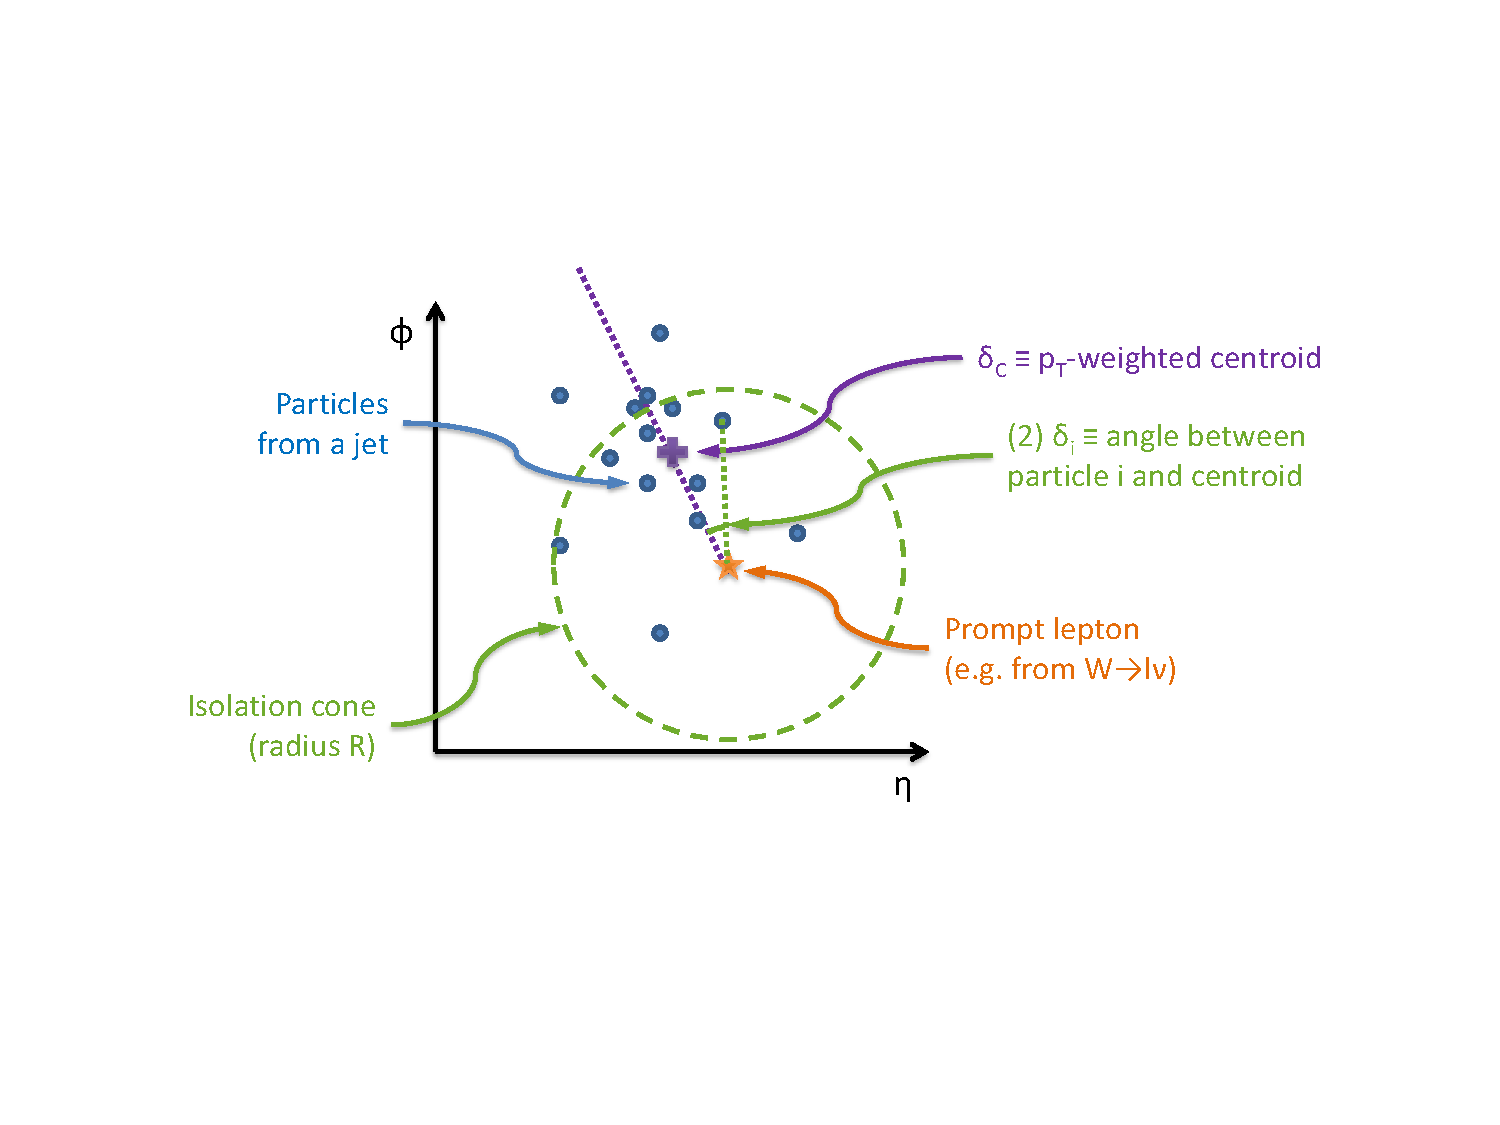
\includegraphics[width=0.8\textwidth]{figures/eventreco_objects/directional_iso_cartoon}
  \caption{Illustration of ingredients used in the computation of directional isolation for a prompt
muon, denoted by a star, near some particles from a jet, denoted by points, in the $(\eta,\phi)$
plane. For prompt leptons $\delta_i$ tends to be small, especially for the high-\pt particles near
the core of the jet. Figure taken from Ref.~\cite{CMS-AN2011-498}.
  \label{fig:object_directional_iso}}
\end{figure}

Apart from the isolation, the identication criteria themselves are also altered from the standard
Loose Muon ID from the POG in order to further optimize the muon identification in environments
with large hadronic activity. 
Loose muons are reconstructed using either the global muon algorithm or the tracker-only
algorithm. 
Global muons are required to pass the {\tt GlobalMuonPromptTight} quality criteria,
and to have at least two muon chambers containing segments uniquely matched to its inner track. 
Tracker-only muons are required to pass the {\tt TMLastStationTight} criteria, which require the
muon to have compatible hits in the last muon chamber. 
All selected muons are then required to pass the selection listed in
Table~\ref{tab:object_loosemuon}. 
Some aspects of the selection depend on the muon $\pt$ and $\eta$; these are summarized in
Table~\ref{tab:object_loosemuon_cuts}.

\begin{table}[p]
\caption{Loose muon definition. }
\begin{center}
{\small
\begin{tabular}{l l}
\toprule
\pt & $> 5\GeV$ \\
$|\eta|$ & $< 2.4$ \\
\midrule
\texttt{\footnotesize innerTrack().hitPattern().numberOfLostHits()} & $\leq 1$ if $\pt < 20\GeV$ \\
                                                      & $\leq 4$ if $\pt \geq 20\GeV$ \\
$|\texttt{\footnotesize innerTrack().dxy(vertex.position())}|$ & $\pt$- and $\eta$-dependent\\
$|\texttt{\footnotesize muonBestTrack().dz(vertex.position())}|$ & $\pt$- and $\eta$-dependent\\
\midrule
$\overrightarrow{\mathrm{ISO}}(R=0.2)$ & $\pt$- and $\eta$-dependent \\
\bottomrule
\end{tabular}
}
\end{center}
\label{tab:object_loosemuon}
\end{table}

\begin{table}[p]
\caption{Details of the $\pt$ dependent thresholds employed in the loose muon selection.}
\begin{center}
  \begin{tabular}{l cccccc }
      \toprule
      Muon $\pt$  & $d_{xy} (\cm)$ & $d_{xy} (\cm)$ & $d_z (\cm)$ & $d_z (\cm)$ &
$\overrightarrow{\mathrm{ISO}}(0.2)$ &
$\overrightarrow{\mathrm{ISO}}(0.2)$ \\
      (\GeV) & Barrel & Endcap & Barrel & Endcap & Barrel & Endcap \\
      \midrule
      0 - 5          & 0.052 & 0.037 & 0.054 & 0.076 & 1.5  & 2    \\
      5 - 10         & 0.041 & 0.018 & 0.042 & 0.082 & 3    & 2.5  \\
      10 - 25        & 0.029 & 0.013 & 0.028 & 0.098 & 7    & 7.5  \\
      15 - 20        & 0.014 & 0.015 & 0.034 & 0.1   & 10.5 & 9    \\
      20 - 40        & 0.021 & 0.021 & 1     & 0.1   & 15.5 & 13.5 \\
      40 - 80        & 0.04  & 0.2   & 1     & 1     & 32.5 & 19   \\
      80 - 140       & 0.1   & 0.2   & 1     & 1     & 54.5 & 37   \\
      140 - 200      & 0.1   & 0.2   & 1     & 1     & 87   & 65.5 \\
      \bottomrule
    \end{tabular}
\end{center}
\label{tab:object_loosemuon_cuts}
\end{table}

 
The \textbf{tight muon selection} follows the recommendation from the Muon POG~\cite{MuonID}.
In addition to the identification criteria, we also require the tight muon to be isolated. 
Here we do not use directional isolation, but rather the more standard particle-based relative
isolation. 
This isolation, denoted $I_\mu$, is calculated using the PF candidates in a cone of size $\Delta R =
0.4$ around the muon. Charged-hadron candidates associated with pileup vertexes are not taken into
account in the calculation of the isolation. However, they are used to estimate the remaining
contribution to the isolation coming from neutral hadrons associated with pileup. This contribution
is then subtracted. 
The isolation definition is given by:
\begin{equation}
I_\mu = \frac{I_{Charged} + I_{Neutral} + I_{\gamma} - \Delta\beta\cdot I_{Charged}^{PU}}
             {\pt^\mu} , 
\label{eqn:iso}
\end{equation}
where $I_{Charged}$, $I_{Neutral}$, and $I_{\gamma}$ are computed as the sum of the \pt of the
charged hadrons, neutral hadrons and photons, respectively, in a cone of size $\Delta R = 0.4$
around the muon. The parameter $\Delta\beta$ is set to 0.5, and $I_{Charged}^{PU}$ is the estimated
contribution from pileup computed as the sum of the \pt of the charged hadrons associated with
pileup vertices.
The tight muon isolation requirement is $I_\mu < 0.15$.
A summary of the tight muon selection can be found in Table~\ref{tab:object_tightmuon}. 

\begin{table}[p]
\caption{Tight muon definition. }
\begin{center}
{\small
\begin{tabular}{l l}
\toprule
\pt & $> 10\GeV$ \\
$|\eta|$ & $< 2.4$ \\
\midrule
\texttt{\footnotesize isPFMuon()} & $= 1$ \\
\texttt{\footnotesize isGlobalMuon()} & $= 1$ \\
\texttt{\footnotesize globalTrack().normalizedChi2()} & $< 10$ \\
\texttt{\footnotesize globalTrack().hitPattern().numberOfValidMuonHits()} & $> 0$ \\
\texttt{\footnotesize track().hitPattern().trackerLayersWithMeasurement()} & $> 5$ \\
\texttt{\footnotesize innerTrack().hitPattern().numberOfValidPixelHits()} & $> 0$ \\
\texttt{\footnotesize numberOfMatchedStations()} & $> 1$ \\
$|\texttt{\footnotesize innerTrack().dxy(vertex.position())}|$ & $< 0.2\cm$ \\
$|\texttt{\footnotesize muonBestTrack().dz(vertex.position())}|$ & $< 0.5\cm$ \\
\midrule
$I_\mu =$ [\texttt{\footnotesize pfIsolationR04().sumChargedHadronPt()}& \\
\hspace{0.9cm} $+$ max(0., \texttt{\footnotesize pfIsolationR04().sumNeutralHadronPt()}  & \\
\hspace{2.7cm} $+$ \texttt{\footnotesize pfIsolationR04().sumPhotonPt()}  & \\
\hspace{2.7cm} $-$ 0.5 $\cdot$ \texttt{\footnotesize pfIsolationR04().sumPUPt()}) & \\
\hspace{0.9cm} ] / \pt & $< 0.15$ \\ 
\bottomrule
\end{tabular}
}
\end{center}
\label{tab:object_tightmuon}
\end{table}

 

\subsubsection{Electrons \label{sec:object_electron}}

Similar to the muon selection, we identify electrons using two different working points, a loose
selection, and a tight selection. 

% Currently we mainly use the loose definition in the analysis, both for vetoing, and for selecting
% single electron events for the control regions enriched in TTJets and WJets. The tight selection
% is only used to define a control region enriched in $Z\rightarrow ll$ events, from which we
% derive a systematic uncertainty on the predicted number of $Z\rightarrow\nu\nu$ events in our
% signal region.


The \textbf{loose electron selection} uses directional isolation as described in the previous
section, and fully documented in Ref.~\cite{CMS-AN2011-498}. A summary of the complete
loose electron selection is given in Table~\ref{tab:object_looseelectron}, with the details of
the $\pt$- and $\eta$-dependent requirements listed in Table~\ref{tab:object_looseelectron_cuts}. 

\begin{table}[p]
  \caption{Loose electron definition.}
  \begin{center}
  {\small 
    \begin{tabular}{l l l l}
      \toprule
      & Condition & Barrel & Endcap \\
      \midrule
      \pt & & $ > 5 \GeV$ & $> 5\GeV$ \\
      $|\eta|$ & & $ < 1.442$ & $1.556 - 2.5$ \\
      \midrule
      \texttt{\footnotesize gsfTrack().numberOfLostHits()} & $\pt < 20\GeV$ & $= 0$ & $= 0$ \\
      \texttt{\footnotesize gsfTrack().hitPattern().numberOfValidPixelHits()} & $\pt < 10\GeV$ &
$\geq 2$ & $\geq 1$ \\
      $|\texttt{\footnotesize gsfTrack().dz(vertex.position())}|$ & & \multicolumn{2}{l}{$\pt$- and
$\eta$-dependent}\\
      \midrule
      $\overrightarrow{\mathrm{ISO}}(R=0.3)$, calculated from charged particles only & &
\multicolumn{2}{l}{$\pt$- and $\eta$-dependent} \\
      $\overrightarrow{\mathrm{ISO}}(R=0.2)$, barrel only, calculated using all particles & &
\multicolumn{2}{l}{$\pt$- and $\eta$-dependent} \\
      \bottomrule
    \end{tabular}
    }
  \end{center}
  \label{tab:object_looseelectron} 
\end{table}


\begin{table}[p]
  \caption{Details of the $\pt$ dependent thresholds employed in the loose electron selection.}
  \begin{center}
  \begin{tabular}{ l ccccc }
      \toprule
      Electron $\pt$ & $d_z (\cm)$ & $d_z (\cm)$ &
$\overrightarrow{\mathrm{ISO}}(0.3,\textrm{charged})$ &
$\overrightarrow{\mathrm{ISO}}(0.3,\textrm{charged})$ & $\overrightarrow{\mathrm{ISO}}(0.2)$ \\
      (\GeV) & Barrel & Endcap & Barrel & Endcap & Barrel \\
      \midrule
      0 - 5          & 0.03 & 0.09 & 0.5  & 0.5  & 2    \\
      5 - 10         & 0.05 & 0.09 & 1.5  & 2.5  & 4.25 \\
      10 - 25        & 0.05 & 0.09 & 4.5  & 6.5  & 8.75 \\
      15 - 20        & 0.05 & 0.11 & 7.5  & 9    & 11   \\
      20 - 40        & 0.2  & 1    & 10   & 10.5 & 20.8 \\
      40 - 80        & 1    & 1    & 18.5 & 18.5 & 200  \\
      80 - 140       & 1    & 1    & 44   & 66.5 & 200  \\
      140 - 200      & 1    & 1    & 81.5 & 70   & 200  \\
      \bottomrule
    \end{tabular}
  \end{center}
  \label{tab:object_looseelectron_cuts}
\end{table}

The \textbf{tight electron selection} is in accordance with the recommendations of the EGamma POG
\cite{ElectronID}. A summary of the selection can be found in table~\ref{tab:object_tightelectron}.
We also require to electron to be isolated. The isolation is calculated using the PF candidates in a
cone of size $\Delta R = 0.3$ around the electron, and then corrected with an estimate of the
median energy from pileup as calculated with the {\tt FastJet} algorithm in a similar way to the
jet corrections explained in Sec.~\ref{sec:object_jets}. We require that this corrected isolation,
relative to the $\pt$ of the electron is less than 0.15.

\begin{equation}
I_e = \frac{ I_{Charged} + \max(0, I_{NeutralHad} + I_{\gamma} - A \rho ) }{\pt^e}
\end{equation}

% TODO: add more info on the pileup correction

\begin{table}[p]
\caption{Tight electron definition. }
\begin{center}
{\small
\begin{tabular}{l l l}
\toprule
& Barrel & Endcap \\
\midrule
\pt & $> 10\GeV$ & $> 10\GeV$\\
$|\eta|$ & $< 1.442$ & $1.556 - 2.5$ \\
\midrule
$|$\texttt{\footnotesize deltaEtaSuperClusterTrackAtVtx()}$|$ & $< 0.004$ & $< 0.005$ \\
$|$\texttt{\footnotesize deltaPhiSuperClusterTrackAtVtx()}$|$ & $< 0.030$ & $< 0.020$ \\
\texttt{\footnotesize sigmaIetaIeta()} & $< 0.010$ & $< 0.030$ \\
\texttt{\footnotesize hadronicOverEm()} & $< 0.120$ & $< 0.100$ \\
1.0/\texttt{\footnotesize ecalEnergy()} - \texttt{\footnotesize eSuperClusterOverP()/ecalEnergy()} &
$< 0.050$ &
$< 0.050$ \\
\texttt{\footnotesize gsfTrack().trackerExpectedHitsInner().numberOfHits()} & $\le 0$ & $\le 0$ \\
\texttt{\footnotesize passConversionVeto()} & $= 1$ & $= 1$ \\
$|\texttt{\footnotesize innerTrack().dxy(vertex.position())}|$ & $< 0.02\cm$ & $< 0.02\cm$\\
$|\texttt{\footnotesize gsfTrack().dz(vertex.position())}|$ & $< 0.1\cm$ & $< 0.1\cm$ \\
\midrule
$I_e$ & $<0.15$ & $< 0.15$ \\
\bottomrule
\end{tabular}
}
\end{center}
\label{tab:object_tightelectron}
\end{table}


\subsubsection{Isolated tracks \label{sec:object_isolatedtrack}}

In order to suppress the decays of both taus and other leptons that do not pass the loose
selection, we can veto events for which an isolated track is present~\cite{CMS-AN2013-089}. 
Isolated tracks are selected from the charged PF candidates with $\pt > 10\GeV$ and
longitudional track-primary vertex distance of $d_z < 0.05\cm$. They are required to have a
relative isolation in a cone of $\Delta R = 0.3$ of less than 0.1. 
In the razor boost analysis the isolated track veto will only be applied in the hadronic event
selections, and not in the control regions which require the presence of a lepton. 

\begin{table}[htdp]
\caption{Isolated track selection. }
\begin{center}
\begin{tabular}{l l}
\toprule
\pt & $> 10\GeV$ \\
\midrule
\texttt{charge()} & $> 0$ \\
$d_z({\rm PV, track})$ & $< 0.05\cm$ \\
$I_{\textrm{track}_i} = \frac{\sum_{j \neq i} \pt{}_j }{ \pt{}_i }$ & $< 0.1$ \\
\bottomrule
\end{tabular}
\end{center}
\label{tab:isolatedtrack}
\end{table}

\subsubsection{Missing transverse momentum \label{sec:object_met}}

The missing transverse momentum, \ETm, associated with a given event is computed as the negative
vector sum of the transverse momentum of all PF candidates $i$,
\begin{equation}
  \ETm = - \sum_i \pt^i .
\end{equation}
The corrections to the jet energy scale discussed above are propagated to the \ETm as well. 
Within CMS this type of missing transverse momentum is know as type-1 corrected \ETm.

No explicit selection will be placed on \ETm in the razor boost analysis selection, although it is
used in the definition of the razor variable $\rsq$, to be introduced in
Section~\ref{sec:boost_razor}.

